\documentclass[11pt,letterpaper]{article}
\usepackage[utf8]{inputenc}
\usepackage{amsmath,amssymb,fullpage,graphicx}
\usepackage{afterpage}

\begin{document}
\subsection*{Lect 12-4}
\subsection*{a}
\begin{verbatim}
p <- 5
y.m <- matrix(0, ncol = 5, nrow = 5)
y.m[1,] <- c(8, 7, 1, 7, 3)
y.m[2,] <- c(11, 2, 7, 3, 8)
y.m[3,] <- c(4, 9, 10, 1, 5)
y.m[4,] <- c(6, 8, 6, 6, 10)
y.m[5,] <- c(4, 2, 3, 8, 8)
treatment <- matrix('A', ncol = 5, nrow = 5)
treatment[1,] <- c('A', 'B', 'D', 'C', 'E')
treatment[2,] <- c('C', 'E', 'A', 'D', 'B')
treatment[3,] <- c('B', 'A', 'C', 'E', 'D')
treatment[4,] <- c('D', 'C', 'E', 'B', 'A')
treatment[5,] <- c('E', 'D', 'B', 'A', 'C') 

bar_yi.. <- apply(y.m, 1, mean)
bar_y..k <- apply(y.m, 2, mean)
bar_y.j. <- as.vector(c(mean(y.m[treatment=='A']), mean(y.m[treatment=='B']),
                        mean(y.m[treatment=='C']), mean(y.m[treatment=='D']), 
                        mean(y.m[treatment=='E']) ))
grand_mean <- mean(y.m)
SSA <- p * sum((bar_yi.. - grand_mean)^2)
SSB <- p * sum((bar_y.j. - grand_mean)^2)
SSC <- p * sum((bar_y..k - grand_mean)^2)
SST <- sum((as.vector(y.m) - grand_mean)^2)
SSE <- SST - SSA - SSB - SSC

F_ratio_A <- (SSA / (p-1)) / (SSE / ((p-1)* (p-2)))
p_value_A <- pf(F_ratio_A, df1=(p-1), df2=(p-1) * (p-2), lower.tail = F)

F_ratio_B <- (SSB / (p-1)) / (SSE / ((p-1)* (p-2)))
p_value_B <- pf(F_ratio_B, df1=(p-1), df2=(p-1) * (p-2), lower.tail = F)

F_ratio_C <- (SSC / (p-1)) / (SSE / ((p-1)* (p-2)))
p_value_C <- pf(F_ratio_C, df1=(p-1), df2=(p-1) * (p-2), lower.tail = F)
\end{verbatim}

\noindent \textbf{SSA, SSB, SSC SSE, SST and corresponding F-ration and p-values are shown below}

\begin{verbatim}
> c(SSA, SSB, SSC, SSE, SST)
[1]  15.44 141.44  12.24  37.52 206.64

> SSA
[1] 15.44
> F_ratio_A
[1] 1.234542
> p_value_A
[1] 0.3476182

> SSB
[1] 141.44
> F_ratio_B
[1] 11.30917
> p_value_B
[1] 0.0004876512

> SSC
[1] 12.24
> F_ratio_C
[1] 0.978678
> p_value_C
[1] 0.4550143
\end{verbatim}


\subsection*{b}
\begin{verbatim}
y <- as.vector(t(y.m))
A <- as.factor(rep(c(1:p), each=p))
C <- as.factor(rep(c(1:p), times=p))
B <- as.factor(as.vector(t(treatment)))
summary.aov(lm(y~A+B+C))

            Df Sum Sq Mean Sq F value   Pr(>F)    
A            4  15.44    3.86   1.235 0.347618    
B            4 141.44   35.36  11.309 0.000488 ***
C            4  12.24    3.06   0.979 0.455014    
Residuals   12  37.52    3.13                     
---
\end{verbatim}

\noindent $SSA = 15.44, SSB = 141.44, SSC = 12.24, SSE = 37.52, SST = 206.64$ \\

\noindent F-ratios for A, B, C are $1.235, 11.309, 0.979$, p-values for A,B,C are $0.34, 0.000488, 0.455$ \\

\noindent Results in part a and part b are same. 

\subsection*{Lect 12-5}
\begin{verbatim}
p <- 4
y.m2 <- matrix(0, ncol = 4, nrow = 4)
y.m2[1,] <- c(11, 10, 14, 8)
y.m2[2,] <- c(8, 12, 10, 12)
y.m2[3,] <- c(9, 11, 7, 15)
y.m2[4,] <- c(9, 8, 18, 6)

treatment1 <- matrix(0, ncol = 4, nrow = 4)
treatment1[1,] = c(3,2,4,1)
treatment1[2,] = c(2,3,1,4)
treatment1[3,] = c(1,4,2,3)
treatment1[4,] = c(4,1,3,2)

treatment2 = matrix(0, ncol = 4, nrow = 4)
treatment2[1,] = c(2,3,4,1)
treatment2[2,] = c(1,4,3,2)
treatment2[3,] = c(4,1,2,3)
treatment2[4,] = c(3,2,1,4)

y <- as.vector(t(y.m2))
A <- as.factor(rep(c(1:p), each=p))
B <- as.factor(rep(c(1:p), times=p))
t1 <- as.factor(as.vector(t(treatment1)))
t2 <- as.factor(as.vector(t(treatment2)))

summary.aov(lm(y~A+B+t1+t2))

            Df Sum Sq Mean Sq F value Pr(>F)
A            3    0.5    0.17   0.018  0.996
B            3   19.0    6.33   0.691  0.616
t1           3   95.5   31.83   3.473  0.167
t2           3    7.5    2.50   0.273  0.843
Residuals    3   27.5    9.17           
\end{verbatim}

\noindent Base on ANOVA table of GLSD, p-value of both treatment factors are greater than $0.05$, implying the data is insignificant to provide evidence against the null hypothesis. The treatment factors may not have effect. 

\afterpage{\null\newpage}
\newpage

\subsection*{Lect 14-3}
\begin{verbatim}
y <- c(6,5,6,5,3,2,4,1,10,9,11,11,10,9,9,10)
FF <- as.factor(rep(c(1,2), each=8))
BB <- as.factor(rep(c(1,1,2,2), time=4))
WW <- as.factor(rep(c(rep(1,time=4), rep(2,time=4)), time=2))

predicts <- predict(lm(y~FF + BB + WW + FF:BB + FF:WW + BB:WW + FF:BB:WW))
residuals <- y - predicts

qqnorm(residuals, ylab='Residuals')

par(mfrow=c(2,2))
plot(x=predicts, y=residuals, xlab='Predicted value')
abline(h=0, lty=2)
plot(as.vector(x=FF), y=residuals, xlab='Factor one')
abline(h=0, lty=2)
plot(as.vector(x=BB), y=residuals, xlab='Factor two')
abline(h=0, lty=2)
plot(as.vector(x=WW), y=residuals, xlab='Factor three')
abline(h=0, lty=2)

\end{verbatim}

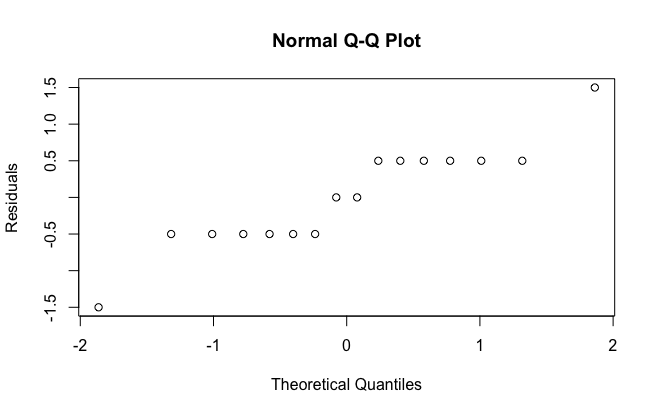
\includegraphics[scale=0.55]{lect-14-3-b-qqplot.png}

\noindent The qqplot of residuals didn't show an obvious shape of line, since there are only 5 levels of residual value. It is hard to say if normality assumption is violated or not. 

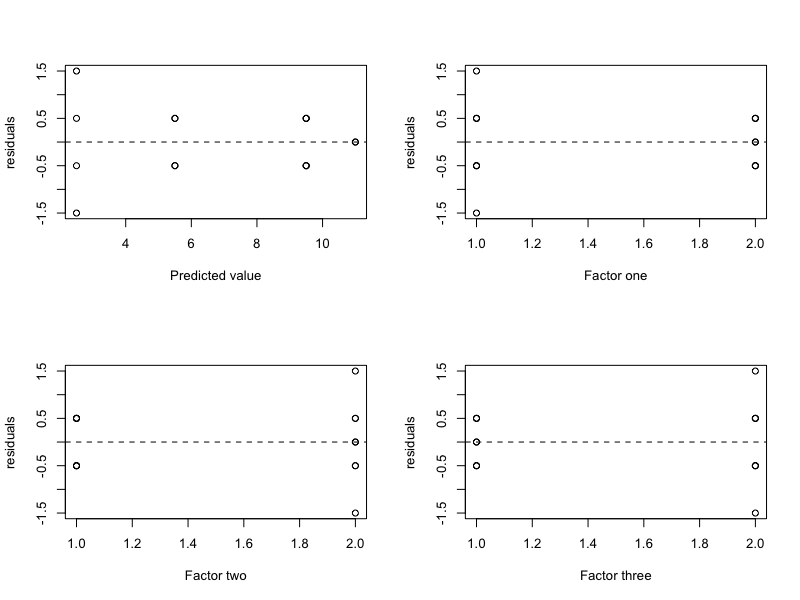
\includegraphics[scale=0.55]{lect-14-3-b-residualplot.png}

\noindent All of the residual plots do not have specific shapes, therefore, equal variance assumption is not violated. 


\subsection*{c}
\begin{verbatim}
y2 <- y^1.7
predicts2 <- predict(lm(y2~FF + BB + WW + FF:BB + FF:WW + BB:WW + FF:BB:WW))
residuals2 <- y2 - predicts2

qqnorm(residuals2)

par(mfrow=c(2,2))
plot(x=predicts2, y=residuals2, xlab='Predicted value')
abline(h=0, lty=2)
plot(as.vector(x=FF), y=residuals2, xlab='Factor one')
abline(h=0, lty=2)
plot(as.vector(x=BB), y=residuals2, xlab='Factor two')
abline(h=0, lty=2)
plot(as.vector(x=WW), y=residuals2, xlab='Factor three')
abline(h=0, lty=2)
\end{verbatim}

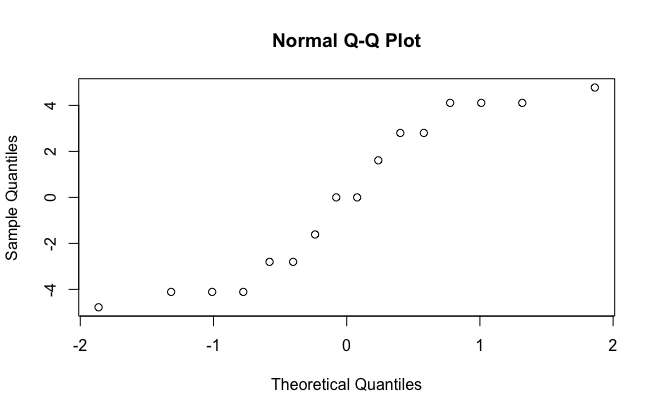
\includegraphics[scale=0.55]{lect-14-3-c-qqplot.png}

\noindent The qqplot seems to have the shape of line, implying the normality assumption is not violated. 

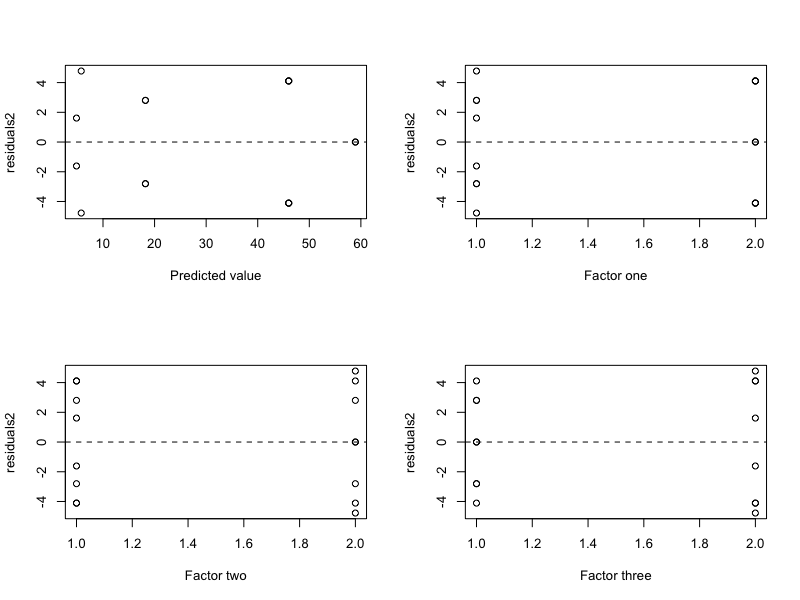
\includegraphics[scale=0.55]{lect-14-3-c-residualplot.png}

\noindent Residual plots are randomly distributed across x=0, having no obvious shape. This implies the equal variance assumption is not violated. 

\newpage
\subsection*{Lect 14-4}
\subsection*{a}
\begin{verbatim}
rm(list=ls(all=TRUE))
y <- c(-35,-45,-40,17,-65,20,-39,-55,15,110,-10,80,55,-55,110,90,-28,110,
       4,-40,31,-23,-64,-20,-30,-61,54)
factors <- gen.factorial(c(3,3,3), varNames = c('Speed', 'Nozzle_Type', 'Pressure'), factors = 'all')
attach(factors)
lm2 <- lm(y~Nozzle_Type + Speed + Pressure + Nozzle_Type:Speed + Nozzle_Type:Pressure + Speed:Pressure)
summary.aov(lm2)

                     Df Sum Sq Mean Sq F value   Pr(>F)    
Nozzle_Type           2    480     240   0.506 0.620709    
Speed                 2  36474   18237  38.481 7.86e-05 ***
Pressure              2  31634   15817  33.375 0.000131 ***
Nozzle_Type:Speed     4   3399     850   1.793 0.223418    
Nozzle_Type:Pressure  4   3729     932   1.967 0.192726    
Speed:Pressure        4   7626    1906   4.023 0.044649 *  
Residuals             8   3791     474                   
---
\end{verbatim}

\noindent Base on the ANOVA table, factors speed and pressure may have significant effects, since the sum of square's of speed and pressure are relatively large. Beside these two factors, the interaction between speed and pressure is also significant, comparing to other two interactions. Factor Nozzle type doesn't seem to have significant effect for its sum of square is relatively small. 

\subsection*{b}
\begin{verbatim}
data_full <- data.frame(y, Nozzle_Type, Speed, Pressure)
Nozzle_Type2 <- as.factor(rep(c(1,2,3), time=3))
Speed2 <- as.factor(rep(c(1,2,3), each=3))
Pressure2 <- as.factor(c(1,2,3,2,3,1,3,1,2))
y2 <- numeric(9)
for (i in 1:9) {
  index1 <- as.numeric(as.vector(Nozzle_Type2)[i])
  index2 <- as.numeric(as.vector(Speed2)[i])
  index3 <- as.numeric(as.vector(Pressure2)[i])
  y2[i] <- data_full[Nozzle_Type==index1 & Speed==index2 & Pressure==index3,1]
}

lm3 <- lm(y2~Nozzle_Type2 + Speed2 + Pressure2)
summary.aov(lm3)

             Df Sum Sq Mean Sq F value Pr(>F)  
Nozzle_Type2  2    260     130   0.591 0.6285  
Speed2        2  14167    7083  32.181 0.0301 *
Pressure2     2  10911    5455  24.785 0.0388 *
Residuals     2    440     220                 
---
\end{verbatim}

\noindent In this LSD, it turns out factors Speed and Pressure have significant effects, and factor Nozzle Type doesn't have significant effect. \\

\noindent The conclusion in part b is consistent with conclusion in part a.

\subsection*{c}
\begin{verbatim}
lm4 <- lm(y2~Nozzle_Type2 + Speed2 + Pressure2 + Speed2:Pressure2)
summary.aov(lm4)

                 Df Sum Sq Mean Sq
Nozzle_Type2      2    260     130
Speed2            2  14167    7083
Pressure2         2  10911    5455
Speed2:Pressure2  2    440     220
\end{verbatim}

\noindent In this case, the parameters over-number independent equations which leads to zero-value of SSE. Therefore, we are unable to do F test. 

\end{document}